%\documentclass{article}
\documentclass[twocolumn]{article}
\usepackage[utf8]{inputenc}
\usepackage{tikz}
\usetikzlibrary{positioning,fit,shapes,arrows.meta}

\author{
	K\'evin Le Bon
	\and
	Alan Schmitt
}

\title{MLExplain}

\begin{document}
\maketitle

\begin{abstract}
	MLExplain is a step-by-step visual interpreter for OCaml that enables the user
	to inspect both their program's state and the interpreter's state itself. This interpreter
	aims to provide the user with a better understanding of the semantics of OCaml.
\end{abstract}

\section{Introduction}

The semantics of a programming language can be very complex. When a language has no specification,
the semantics is then defined by the implementations of the language, i.e., interpreters and
compilers. However even when a specification is available, it can be difficult to understand why
the execution of a specific program results to a certain output.

The project \emph{JSExplain} \cite{chargueraud:hal-01745792} aims to describe
a JavaScript program's execution by showing every step of an interpreter which behavior is the
closest to JavaScript specification. This paper shows how we adapted JSExplain to OCaml.

Unlike JavaScript, OCaml has no official specification. However, OCaml code execution is
fairly simple because the amount of language constructions is small. We have written an
interpreter for OCaml's typed abstract syntax tree (AST). This AST is close to source code and
need little transformations but supplies us with resolved names -- which is useful for module and
signatures inclusion and absolutely mandatory for features like named parameters in functions.
The semantic we give to OCaml is higher level than the one described in \emph{ZINC}
\cite{Leroy-ZINC} virtual machine which is at the same level as object code.

\section{The visual interpreter JSExplain}

An interpreter is a program that takes code written in a specific language as input
and execute it. In order to achieve its goal, the interpreter does several analyses ;
here are the most common : lexical analysis, parsing and typing.

We call a \emph{visual interpreter} an interpreter that is able to display the program's state,
the current location in source and local-variable values at each step of the execution as well as
the state of the interpreter itself. JSExplain is a visual interpreter for JavaScript. The aim of
this tool is to enable a user to better understand JavaScript's semantics. JSExplain's interface
highlights the expression of the program currently evaluated as well as the instruction of
the interpreter that is executed.

\section{JSExplain functioning}

JSExplain is a visual interpreter. To display its state, the interpreter is compiled with a
compiler that adds calls to a tracing function. The traced retrieved during the execution of the
program gives many information about the state of the interpreter:

\begin{itemize}
	\item existing variables and their values
	\item return values of functions of the interpreter
\end{itemize}

JSExplain's web interface uses these traces in order to display the program and interpreter state
at every step of the execution.

\subsection{JSExplain's compiler}

% Expliquer que JSExplain est écrit en OCaml et compilé vers JavaScript pour être intégré dans
% la page web qui va avec

JSExplain needs its own OCaml to JavaScript compiler in order to place the calls to
\verb|log_event| which is the tracing function. This function is also used to get the location
of the different syntactical objects in the source file in order to produce code highlighting in
JSExplain's interface.


\begin{figure*}
  \centering
  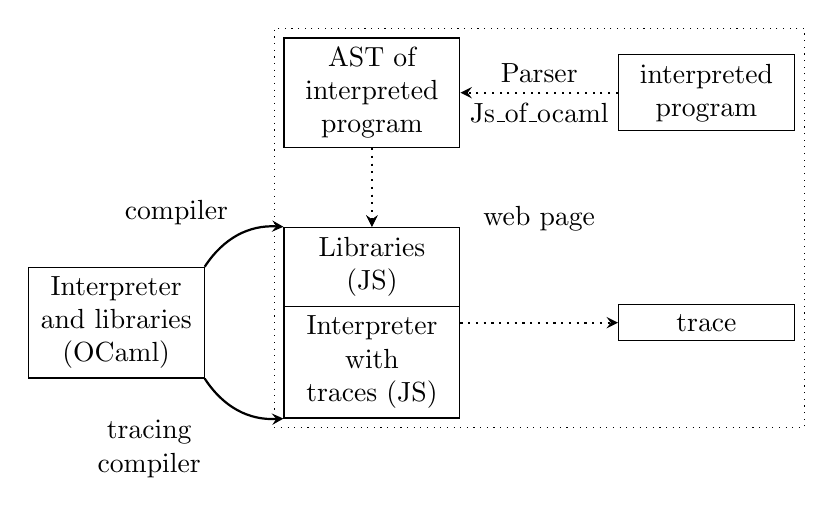
\begin{tikzpicture}[nodes = {align = center}]
    \node (focaml) [draw, text width=2cm] {Interpreter and libraries (OCaml)};

    \node (fjs) [draw, right = 1cm of focaml, text width=2cm, rectangle split,
    rectangle split parts=2, text centered] {Libraries (JS) \nodepart{second}
      Interpreter with traces (JS)};

    \node (ast) [draw, above = of fjs, text width=2cm] {AST of interpreted
      program};

    \node (source) [draw, right = 2cm of ast, text width=2cm, text centered]
    {interpreted program};

    \node [draw, dotted, fit=(fjs) (ast) (source)] {web page};

    \node (trace) [draw, right = 2cm of fjs, text width=2cm, text centered]
    {trace};

    \path[->,thick,>=stealth] (focaml.north
    east) edge[bend left] node[above left] {compiler} (fjs.north west) ;

    \path[->,thick,>=stealth] (focaml.south east) edge[bend right] node[below
    left] {\parbox{2cm}{\centering tracing compiler}} (fjs.south west);

    \path[->,thick,dotted,>=stealth] (source) edge node [above] {Parser} node [below] {Js\_of\_ocaml} (ast);

    \path[->,thick,dotted,>=stealth] (ast) edge (fjs);

    \path[->,thick,dotted,>=stealth] (ast) edge (fjs);

    \path[->,thick,dotted,>=stealth] (fjs) edge (trace);
  \end{tikzpicture}
  
  \caption{Architecture of MLExplain}
  \label{fig:archi}
\end{figure*}

\bibliographystyle{plain}
\bibliography{biblio}

\end{document}
